\section{Empirical Motivation}
\label{sec:motivation}

The conflict between dynamic expert offloading and graph replay is fundamental, but its practical severity remains an empirical question.
If routing rarely changes residency, or if typical working sets fit in bounded HBM, or if transfer latency is negligible, simpler solutions would suffice.
We measure three production MoE architectures spanning 30B to 80B parameters under realistic serving conditions to establish whether the problem demands a new system design.

All measurements use one Ascend 910B2, BF16, tensor parallelism one, disabled prefix caching, and serialized requests (both concurrency controls set to one).\footnote{Qwen3-30B-A3B: 48 routed layers, 128 experts/layer, top-8; GLM-4.7-Flash: 46 routed layers, 64 experts/layer, top-4; Qwen3-Next-80B-A3B-Instruct: 48 routed layers, 512 experts/layer, top-10.}
We profile 200, 100, and 64 ShareGPT requests on Qwen3, GLM, and Qwen3-Next, respectively, generating at most 128 output tokens for Qwen3 and GLM, and 32 for Qwen3-Next to bound collection cost.
An independent audit verifies event-stream integrity, balanced decode sampling, and deterministic reproducibility of all reported statistics.
Figure~\ref{fig:motivation-rewrite} summarizes the key observations.

\begin{figure*}[t]
  \centering
  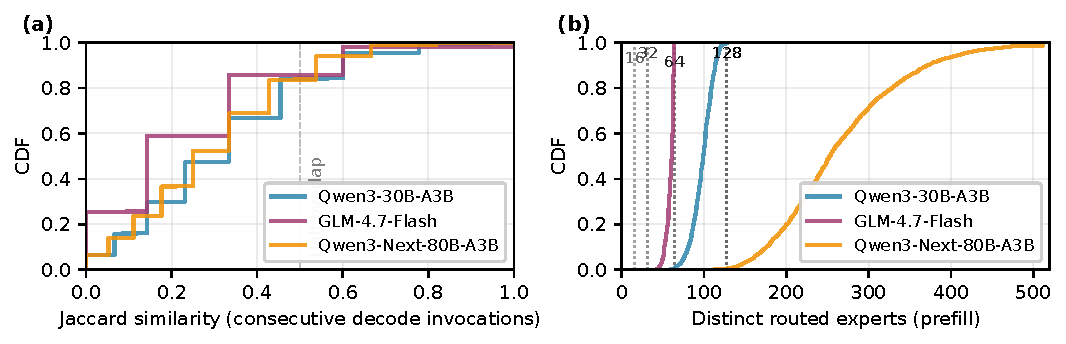
\includegraphics[width=\textwidth]{figures/motivation_rewrite.pdf}
  \Description{Two-panel empirical characterization showing expert turnover across requests and capacity overflow patterns across three MoE models.}
  \caption{%
    Empirical motivation for graph-compatible expert offloading.
    (a) CDF of Jaccard similarity between consecutive prefill invocations within each MoE layer, showing substantial expert turnover across requests.
    Even moderate similarity (e.g., 0.5--0.8) requires frequent mapping updates, as 20--50\% of experts change between invocations.
    (b) CDF of distinct routed experts per prefill invocation.
    Vertical lines mark cache capacities; all three models exhibit working sets that substantially exceed practical capacity bounds.
  }
  \label{fig:motivation-rewrite}
\end{figure*}

\subsection{Expert Residency Changes Frequently Across Requests}

A 32-expert cache serving Qwen3, GLM, and Qwen3-Next experiences cache misses on 20.6\%, 14.0\%, and 38.2\% of decode expert accesses despite sparse activation (8, 4, and 10 experts per layer).
More critically, 68.7\%, 41.0\%, and 94.2\% of layer invocations trigger at least one logical-to-physical mapping update.

Figure~\ref{fig:motivation-rewrite}a quantifies expert turnover across consecutive prefill invocations within each layer.
While Qwen3 and GLM exhibit median Jaccard similarities of 0.78 and 0.92, Qwen3-Next shows substantially lower overlap at 0.54.
Even moderate similarity values translate to frequent residency changes: a Jaccard similarity of 0.78 means 22\% of experts differ between consecutive invocations, and 0.54 means 46\% turnover.
For Qwen3-Next, over 60\% of consecutive invocations share fewer than two-thirds of their experts.

This turnover directly challenges systems that bind captured computation to expert-specific storage locations.
Although sparse activation limits per-token computation, it does not stabilize expert residency.
Each mapping change would require graph recapture under naive storage bindings, negating the host-overhead savings graph replay provides (Figure~\ref{fig:graph_breakdown} in Section~\ref{sec:intro}).

\noindent\textbf{Implication.}
Graph-compatible offloading must decouple logical expert identity from graph-visible storage bindings.
Replay requires stable addresses, not static residency.

\subsection{Working Sets Exceed Practical Cache Capacity}

Prefill aggregates routing decisions across an entire prompt.
Figure~\ref{fig:motivation-rewrite}b shows the distribution of distinct routed experts per prefill invocation, with vertical lines marking cache capacities of 16, 32, 64, and 128 slots.
For a 32-slot cache, \textit{all} 2,400 Qwen3 prefills, \textit{all} 1,100 GLM prefills, and \textit{all} 3,072 Qwen3-Next prefills overflow.
The median active expert counts are 99, 61, and 253; the 95th percentiles reach 117, 64, and 415; maxima span 128, 64, and 512.

Even aggressive capacity scaling provides limited relief.
A 64-slot cache still overflows 99.3\% of Qwen3 prefills and every Qwen3-Next prefill; a 128-slot cache still overflows 99.5\% of Qwen3-Next prefills.
The corresponding median active-weight footprints are 0.87, 1.07, and 1.48~GiB, versus 32-slot budgets of 0.28, 0.56, and 0.19~GiB.
Overflow occurs with a single in-flight request—concurrent batching is not a prerequisite.

\noindent\textbf{Implication.}
A bounded HBM cache must support intra-invocation slot reuse.
Wave-based execution partitions the routed working set while preserving every token--expert pair and its original routing weight.

\subsection{Transfer Latency Justifies Overlap}

Multi-wave execution exposes substantial data movement.
Across profiled prefills, Qwen3, GLM, and Qwen3-Next execute 8,571, 2,200, and 26,695 waves, transferring 1.58, 0.60, and 4.62~TB from host memory.
Even with prefetching, aggregate staging wait accounts for 20.2\%, 24.0\%, and 17.2\% of the corresponding MLP computation time.

\noindent\textbf{Implication.}
Transfer--compute overlap is essential for practical performance.
Sequential wave execution would expose staging latency on every prefill's critical path.
However, asynchronous overlap requires careful coordination between transfer readiness, computation completion, and slot reuse.
Section~\ref{sec:design_lease} describes our versioned lease protocol to ensure correctness when these events advance on independent streams.

\vspace{0.5em}
\noindent
These observations establish three requirements: stable storage bindings despite frequent remapping (\S\ref{sec:design_slots}), bounded-capacity execution despite oversized working sets (\S\ref{sec:design_waves}), and safe asynchronous overlap despite concurrent slot reuse (\S\ref{sec:design_lease}).
